\documentclass[twoside]{article}

% Géométrie de la page :
\usepackage{geometry}
\geometry{paperwidth=7.5cm, paperheight=11cm, inner=0.8cm, outer=0.8cm, tmargin=0.5cm, bmargin=1cm, includehead}

% Choix d'une police principale :
\usepackage{luatextra}
\setmainfont{Arno Pro}

% Redéfinition de la taille des polices :
%\renewcommand{\small}{\fontsize{8}{10}\selectfont}

% Césures etc. :
\usepackage[latin, frenchb]{babel}
\selectlanguage{frenchb}

% Mise en forme des titres de sections :
\usepackage[explicit]{titlesec}
\titleformat{\section}{}{}{0cm}{
    \fontsize{11}{12}\selectfont
    \begin{center}
    \makebox[5.9cm][c]{\centering\textsc{\textbf{#1}}}
    \end{center}
    \vspace{0.2cm}
}
\titlespacing{\section}{0cm}{0cm}{-.5cm}

% Textes en parallèle :
%\usepackage{parallel}

% Entêtes et pieds de pages :
\usepackage{fancyhdr}
\pagestyle{fancy}
\fancyhead{}
\fancyhead[CE]{\fontsize{8}{10}\selectfont\textsc{Benedictiones}}
\fancyhead[CO]{\fontsize{8}{10}\selectfont\textsc{\rightmark}}
\fancyfoot[CE,CO]{\fontsize{8}{10}\selectfont\thepage}
\renewcommand{\sectionmark}[1]{\markright{#1}}
\renewcommand{\headrulewidth}{0.3pt}
\renewcommand{\footrulewidth}{0pt}
\renewcommand{\headrule}{\vbox to 6pt{\hbox to\headwidth{\hrulefill}\vss}}
\setlength{\parindent}{0cm}
\setlength{\headsep}{0.2cm} % Distance entre le header et le corps du texte.
\setlength{\footskip}{0.6cm} % Distance entre le footer et le corps du texte.
% Redéfinition du style {plain} (seulement pied de page) :
\fancypagestyle{plain}{
\fancyhf{}% Clear all.
\fancyfoot[CE,CO]{\fontsize{8}{10}\selectfont\thepage}
\renewcommand{\headrulewidth}{0pt}
\renewcommand{\headrule}{}
\setlength{\headsep}{0cm}
}
% Redéfintion du style {headings} (seulement entête) :
\fancypagestyle{headings}{
\fancyhf{}% Clear all.
\fancyhead[CE]{\fontsize{8}{10}\selectfont\textsc{Benedictiones}}
\fancyhead[CO]{\fontsize{8}{10}\selectfont\textsc{\rightmark}}
\setlength{\footskip}{0cm}
}

% Pour forcer l'usage des césures (cf. mail Thierry Masson) :
\pretolerance = -1
\tolerance = 2000

% Pour augmenter l'approche des caractères :
\usepackage{soul}

% Gregorio :
\usepackage[autocompile]{gregoriotex}
%\grechangedim{commentaryraise}{.4cm}{scalable}
%\grechangestyle{modeline}{\small\scshape}

% Table des matières :
\usepackage{tocloft}
% Pour supprimer les numéros de section dans la table des matières,
% on les met dans des boîtes tempo qu'on n'utilise jamais.
% cf. https://tex.stackexchange.com/questions/71123/remove-section-number-toc-entries-with-tocloft/71136#71136
\makeatletter
\renewcommand{\cftsecpresnum}{\begin{lrbox}{\@tempboxa}}
\renewcommand{\cftsecaftersnum}{\end{lrbox}}
\makeatother


% Various (fonts) :
\usepackage{fontspec}
\usepackage{calc}
\usepackage{pifont}
\frenchbsetup{ThinColonSpace=true}
\newfontfamily{\GregPlantin}[BoldFont = GregPlantin Bold,ItalicFont = GregPlantin Italic,BoldItalicFont = GregPlantin Bolditalic]{GregPlantin Regular}
\newfontfamily{\PlantinStd}{Plantin Std}
\newfontfamily{\GaramondPremierPro}[Numbers=OldStyle]{Garamond Premier Pro}
%\newfontfamily{\GaramondPremierProCaption}[Numbers=OldStyle]{GaramondPremrPro-Capt}
%\newfontfamily{\GaramondPremierProMediumCaption}[Numbers=OldStyle]{GaramondPremrPro-MedCapt}
%\newfontfamily{\GaramondPremierProItCaption}[Numbers=OldStyle]{GaramondPremrPro-ItCapt}
%\newfontfamily{\GaramondPremierProIt}{GaramondPremrPro-It}
%\newfontfamily{\GaramondPremierProMediumIt}{GaramondPremrPro-MedIt}
\newfontfamily{\FlavGaramond}{FlavGaramond}
\definecolor{rougeliturgique}{cmyk}{0.15,1,1,0}
\renewcommand{\Rbar}{\textbf{\color{rougeliturgique}\GregPlantin\symbol{164}}}
\renewcommand{\Vbar}{\textbf{\color{rougeliturgique}\GregPlantin\symbol{8730}}}
\renewcommand{\GreDagger}{\textrm{\color{rougeliturgique}\FlavGaramond \symbol{8224}}}
\catcode`\®=\active
\def®{\Rbar}
\catcode`\√=\active
\def√{\Vbar}
\catcode`\©=\active
\def©{\hspace{-1.2ex}}
\catcode`\†=\active
\def†{\GreDagger}
\makeatletter
\def\accentaigucaractere{\makebox[0pt][c]{´}}
\newcommand\accentaigu[1]{\setlength{\@tempdima}{\widthof{#1}}\hbox{#1\kern-0.5\@tempdima\accentaigucaractere\kern0.5\@tempdima}}
\makeatother
\def\espacefine{\hspace{0.035cm}}
\catcode`\ã=\active% Tilde-a
\defã{\accentaigu{æ}}
\catcode`\õ=\active% Tilde-o
\defõ{\accentaigu{œ}}
\catcode`\Ï=\active% Alt-j
\defÏ{\accentaigu{y}}
\catcode`\™=\active% Alt-Maj-t
\def™{\textit{\color{rougeliturgique}T.P.}}
\catcode`\∏=\active% Alt-Maj-p
\def∏{\textit{\color{rougeliturgique}Ps.}}
\catcode`\ı=\active% Alt-Maj-n
\defı{\textup{\color{rougeliturgique}N.}}
\catcode`\€\active% Alt-* (sinon les * des \vspace* sont actives)
\def€{\GreStar}
\def\GreStar{
{\color{rougeliturgique}\tiny\raisebox{1.5ex}{\ding{72}}}
  \relax
}
%\grechangestyle{initial}{\fontsize{28}{36}\color{rougeliturgique}\PlantinStd }
%\newbox\scorebox
%\gresetheadercapture{commentary}{grecommentary}{string}
%\grechangestaffsize{12}
%\grechangedim{afterinitialshift}{2.2mm}{fixed}
%\grechangedim{beforeinitialshift}{3mm}{fixed}
%\let\grevanillacommentary\grecommentary
%\def\grecommentary#1{\grevanillacommentary{#1\kern 0.3mm}}
%\gresetbarspacing{new}
%\grechangedim{bar@maior@standalone@notext}{0.3 cm}{scalable}
%\grechangedim{spacebeforeeolcustos}{0.3 cm}{scalable}
%\grechangedim{baselineskip}{40pt plus 5 pt minus 5 pt}{scalable}

%%%%%%%%%%%%%%%%%%%%%%%%%%%%%%%
% Commandes et environnements :
%%%%%%%%%%%%%%%%%%%%%%%%%%%%%%%

% Espace fine :
\DeclareRobustCommand{\mynobreakthinspace}{%
\leavevmode\nobreak\hspace{0.08em}}
\def~{\mynobreakthinspace{}}

% Style pour les références des partitions :
%\grechangestyle{commentary}{\color{rougeliturgique}\itshape\fontsize{9}{8}\selectfont}

%% Environnement Boîte (espace avant, contenu) :
%\newenvironment{ParBox}[2]{
%    \setlength{\parindent}{0cm}
%    \begin{center}
%    \parbox[t]{14.85cm}{\vspace{#1} #2}
%    \end{center}
%    \par
%}

% Style de paragraphe TitreA :
\newenvironment{TitreA}[1]{
    \setlength{\parindent}{0cm}
    \setlength{\leftskip}{0cm}
    \fontsize{16}{18}\selectfont
    \setlength{\parskip}{-0.3cm}
    \begin{center}
    {\color{rougeliturgique}\MakeUppercase{#1}}
    \end{center}
}

% Style de paragraphe TitreB :
\newenvironment{TitreB}[1]{
    \setlength{\parindent}{0cm}
    \setlength{\leftskip}{0cm}
    \setlength{\parskip}{-0.3cm}
    \fontsize{10}{12}\selectfont
    \begin{center}
    \textsc{#1}
    \end{center}
}

% Style de paragraphe TitreC :
\newenvironment{TitreC}[1]{
    \setlength{\parindent}{0cm}
    \setlength{\leftskip}{0cm}
    \setlength{\parskip}{0cm}
    \fontsize{10}{10}\selectfont
    \begin{center}
    {\color{rougeliturgique}\textsc{#1}}
    \end{center}
}

% Style de paragraphe Normal :
\newenvironment{Normal}[1]{
    \setlength{\parindent}{0cm}
    \setlength{\leftskip}{0cm}
    \setlength{\parskip}{0cm}
    \selectlanguage{latin}
    \fontsize{9}{10}\selectfont#1\par
    \vspace{0.1cm}
}

% Style de paragraphe Rubrique :
\newenvironment{Rubrique}[1]{
    \setlength{\parindent}{0cm}
    \setlength{\leftskip}{0cm}
    \setlength{\parskip}{0cm}
    \fontsize{9}{11}\selectfont
    {\color{rougeliturgique}\textit{#1}}
    \vspace{0.1cm}
}

% Rubriques à l'intérieur d'un texte :
\newcommand{\RubriqueInside}[1]{
{\fontsize{9}{11}\selectfont\textit{\color{rougeliturgique}#1}}
}

% Partoche :
%\newenvironment{Partoche}[1]{
%    \fontsize{12}{12}\selectfont
%    \selectlanguage{latin}
%    \gregorioscore{\FolderData/#1}
%    \selectlanguage{frenchb}
%    \begin{center}
%    \fontsize{11}{12}\selectfont
%    \parbox[t][\height][b]{9cm}{\vspace{-.2cm}\input{Partoches/#1}}\par\vspace{.1cm}
%    \end{center}
%}

% Latin/francais :
\newenvironment{LF}[2]{
    \setlength{\parindent}{0cm}
    \setlength{\leftskip}{0cm}
    \setlength{\parskip}{0cm}
    \selectlanguage{latin}
    \fontsize{9}{10}\selectfont#1\par
    \selectlanguage{frenchb}
    \setlength{\leftskip}{0.3cm}
    \fontsize{8}{9}\selectfont\textit{#2}
    \vspace{0.1cm}
}

% Ligne de séparation :
\newcommand\Ligne{
\vspace{0.2cm}
\begin{center}
\greseparator{2}{10}
\end{center}
}

%% Citation :
%\newenvironment{Citation}[1]{
%    \fontsize{9}{10}\selectfont
%    \hfill\parbox{6cm}{\begin{flushright}#1\end{flushright}}\par
%}

%

%%%%%%%%%%%%%%%%%
% Symboles spéciaux :
%%%%%%%%%%%%%%%%%

% Antienne :
%\catcode`\ø=\active
%\defø{{\fontspec{FlavGaramond} \symbol{8721}}}
% Verset :
\catcode`\ß=\active
\defß{{\fontspec{FlavGaramond} \symbol{8730}}}
% Croix de Malte:
\catcode`\+=\active
\def+{{\fontspec{Menlo} \symbol{10016}}}

%

%%%%%%%%%%%%%%%%%
% Hyphenations :
%%%%%%%%%%%%%%%%%

\hyphenation{al-le-lu-ia}


%%%%%%%%%%%%%%%%%

\begin{document}

\thispagestyle{empty}

\newgeometry{inner=0cm, outer=0cm, tmargin=0.5cm, bmargin=0.2cm}

\begin{center}

    \TitreB{+}

    \fontsize{8}{9}\selectfont

    \vspace{0.5cm}

    \centering{PAX}

    \vspace{0.3cm}

    \TitreA{Rituel}

    \TitreA{des bénédictions}

    \TitreA{de Règle}

    \vspace{0.7cm}

    \centering{
\includegraphics[width=1cm]{blason.jpg}}

    \vspace{0.5cm}

    \TitreB{ABBAYE}

    \vspace{-0.3cm}

    \TitreB{SAINT-JOSEPH de CLAIRVAL}

    \vspace{-0.1cm}

    \TitreB{Flavigny-sur-Ozerain}

    \vspace{-0.3cm}

    \Ligne

    \vspace{0.3cm}

    \fontsize{8}{9}\selectfont

    \centering{\textit{– Pro manuscripto –}}

\end{center}

\restoregeometry

\newpage

\thispagestyle{empty}

\cleardoublepage

\section{Commémoraison des défunts}

\thispagestyle{plain}

\Rubrique{L’Hebdomadier~:}

\LF{Commemorátio ómnium fratrum, familiárium Ordinis nostri, atque benefactórum nostrórum.}{Souvenons-nous de tous les frères et amis de notre Ordre, ainsi que de nos bienfaiteurs.}

\Rubrique{Le Père Abbé~:}

\LF{√ Requiéscant in pace.}{Qu’ils reposent en paix.}

\Normal{® Amen.}

\Rubrique{Le Maître de Chœur~:}

\TitreC{\oldstylenums{Psaume 129}}

\LF{De profúndis clamávi ad te Dómine, € Dómine exáudi vocem meam.}{Du fond de l’abîme je crie vers vous, Seigneur, Seigneur, écoutez ma voix~;}

\LF{Fiant aures tuæ intendéntes~: € in vocem deprecatiónis meæ.}{Que vos oreilles soient attentives aux accents de ma prière !}

\LF{Si iniquitátes observáveris Dómine~: € Dómine, quis sustinébit ?}{Si vous prenez garde à l’iniquité, Seigneur, Seigneur qui pourra subsister devant vous?}

\LF{Quia apud te propitiátio est~: € et propter legem tuam sustínui te, Dómine.}{Mais auprès de vous est le pardon, et à cause de votre loi je vous attends, Seigneur}

\LF{Sustínuit ánima mea in verbo eius~: € sperávit ánima mea in Dómino.}{Mon âme attend, confiante en votre parole~; mon âme a mis son espoir dans le Seigneur.}

\LF{A custódia matutína usque ad noctem~: € speret Israel in Dómino.}{Depuis la veille du matin jusqu’à la nuit, qu’Israël espère dans le Seigneur !}

\LF{Quia apud Dóminum misericórdia~: € et copiósa apud eum redémptio.}{Car auprès du Seigneur est la miséricorde, auprès de lui une surabondante délivrance.}

\LF{Et ipse rédimet Israel, € ex ómnibus iniquitátibus eius.}{C’est lui qui rachètera Israël de toutes ses iniquités.}

\LF{Réquiem ætérnam, € dona eis Dómine,}{Accordez-leur Seigneur le repos éternel,}

\LF{Et lux perpétua, € lúceat eis.}{Et que la lumière perpétuelle € brille pour eux.}

\Ligne

\vspace{0.5cm}

\Rubrique{On peut ajouter, “ad libitum”~:}

\Rubrique{L’Hebdomadier~:}

\LF{√ A porta ínferi.}{Des portes de l’enfer.}

\LF{® Erue, Dómine ánimas eórum.}{Seigneur, délivrez leurs âmes.}

\LF{√ Requiéscant in pace.}{Qu’ils reposent en paix.}

\Normal{® Amen.}

\LF{√ Dómine, exáudi oratiónem meam.}{Seigneur, exaucez ma prière.}

\LF{® Et clamor meus ad te véniat.}{Et que mon cri parvienne jusqu’à vous.}

\LF{√ Dóminus vobíscum.}{Le Seigneur soit avec vous.}

\LF{® Et cum spíritu tuo.}{Et avec votre esprit.}

\LF{\textbf{Orémus} – Deus, véniæ largítor et humánæ salútis amátor~: † quãsumus cleméntiam tuam~; ut nostræ congregatiónis fratres, propínquos, et benefactóres, qui ex hoc sãculo transiérunt, € beáta María semper Vírgine intercedénte cum ómnibus Sanctis tuis, ad perpétuæ beatitúdinis consórtium perveníre concédas. Per Christum Dóminum nostrum.}{Dieu généreux dans le pardon, qui aimez à sauver les hommes~; nous supplions votre clémence~: faites que les frères, les proches et les bienfaiteurs de notre congrégation qui ont quitté ce monde parviennent, par l’intercession de la Bienheureuse Marie toujours Vierge et de tous les Saints, à la possession de la béatitude éternelle. Par le Christ Notre Seigneur.}

\Normal{® Amen.}

\Rubrique{L’Hebdomadier~:}

\LF{√ Réquiem ætérnam dona eis, Dómine.}{Donnez-leur le repos éternel, Seigneur.}

\LF{® Et lux perpétua lúceat eis.}{Et que le lumière sans déclin brille pour eux.}

\LF{√ Requiéscant in pace.}{Qu’ils reposent en paix.}

\Normal{® Amen.}

\vspace{1cm}

\thispagestyle{headings}

\Ligne

\newpage

\thispagestyle{empty}

\begin{center}
    \parbox{5.5cm}{\vspace{0.5cm}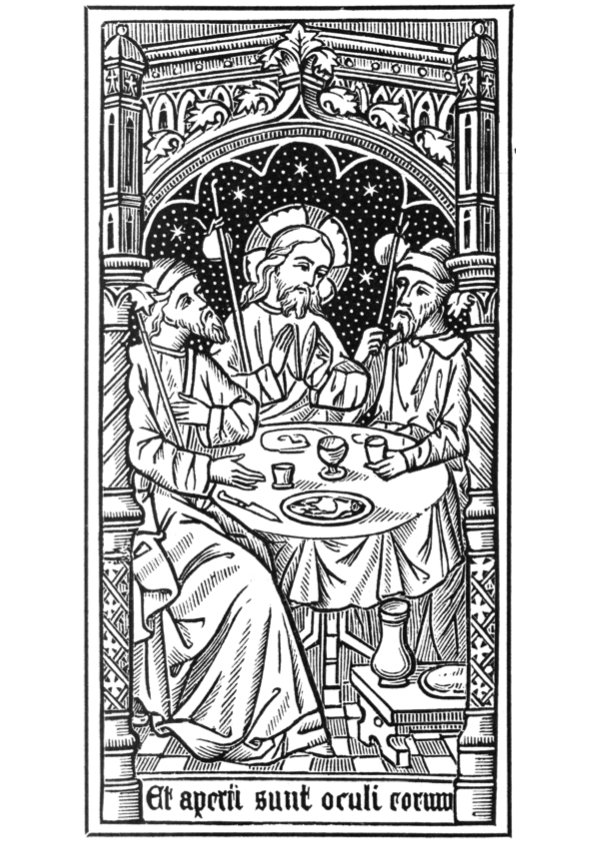
\includegraphics[width=5.5cm]{repas.jpg}}
\end{center}

\section{Temps pendant l'année}

\thispagestyle{plain}

\TitreC{Avant le repas de midi}

\Rubrique{Le Père Abbé~:}

\Normal{√ Benedícite.}

\Normal{® Benedícite.}

\LF{√ Oculi ómnium…}{Les yeux de tous les vivants…}

\LF{® … in te sperant Dómine, † et tu das escam illórum in témpore opportúno, € áperis tu manum tuam et imples omne ánimal benedictióne.}{… espèrent en vous, Seigneur, et vous leur donnez la nourriture en temps opportun~; vous ouvrez votre main et vous comblez tout être vivant de bénédictions.}

\LF{\textbf{Orémus} – Bénedic Dómine nos et hæc tua dona, € quæ de tua largitáte sumus sumptúri. Per Christum Dóminum nostrum.}{Prions - Bénissez-nous, Seigneur, ainsi que ces dons qui sont vôtres et que nous allons recevoir de votre largesse. Par le Christ Notre-Seigneur.}

\Normal{® Amen.}

\Rubrique{Le lecteur~:}

\LF{Iube Domne benedícere.}{Veuillez, mon Père, me bénir.}

\Rubrique{Le Père Abbé~:}

\LF{√ Mensæ cæléstis partícipes € fáciat nos Rex ætérnæ glóriæ.}{Que le Roi d’éternelle gloire nous fasse participants de la table céleste.}

\Normal{® Amen.}

\TitreC{Après le repas de midi}

\Rubrique{Le lecteur~:}

\LF{√ Tu autem Dómine, € miserére nobis.}{Mais vous, Seigneur, ayez pitié de nous.}

\LF{® Deo grátias.}{Nous rendons grâces à Dieu.}

\newpage

\Rubrique{Le Père Abbé~:}

\LF{√ Confiteántur…}{Que toutes vos œuvres…}

\LF{® … tibi, Dómine ómnia ópera tua, et sancti tui benedícant tibi.}{… vous louent, Seigneur, et que vos saints vous bénissent.}

\LF{√ Agimus tibi grátias, omnípotens Deus, † pro univérsis benefíciis tuis € qui vivis et regnas in sǽcula sæculórum.}{Nous vous rendons grâces, ô Dieu tout-puissant, pour tous vos bienfaits, vous qui vivez et régnez pour les siècles des siècles.}

\Normal{® Amen.}

\LF{√ Retribúere dignáre, Dómine, † ómnibus nobis bona faciéntibus propter nomen tuum € vitam ætérnam.}{Seigneur, daignez donner à tous  ceux qui nous font du bien à cause de votre nom, la récompense de la vie éternelle.}

\Normal{® Amen.}

\newpage

\Rubrique{Un chantre~:}

\TitreC{Psaume \oldstylenums{50}\label{psaume_50}}

\LF{Miserére mei Deus, € secúndum magnam misericórdiam tuam~;}{Ayez pitié de moi, ô Dieu, selon votre grande miséricorde,}

\LF{Et secúndum multitúdinem miseratiónum tuárum, € dele iniquitátem meam.}{Et selon l’étendue de vos bontés effacez mes transgressions.}

\LF{Amplius lava me ab iniquitáte mea~: € et a peccáto meo munda me~;}{Lavez-moi de plus en plus de mon iniquité, et purifiez-moi de mon péché~;}

\LF{Quóniam iniquitátem meam ego cognósco~: € et peccátum meum contra me est semper.}{Car je reconnais mes offenses, et mon péché est constamment devant moi.}

\LF{Tibi soli peccávi, et malum coram te feci~: € ut iustificéris in sermónibus tuis, et vincas cum iudicáris.}{C’est contre vous seul que j’ai péché, et j’ai fait ce qui est mal à vos yeux~; (j’en fais l’aveu) afin que vous soyez trouvé juste dans votre sentence, sans reproche dans votre jugement.}

\LF{Ecce enim in iniquitátibus concéptus sum~: € et in peccátis concépit me mater mea.}{Je suis né dans l’iniquité, et ma mère m’a conçu dans le péché.}

\LF{Ecce enim veritátem dilexísti~: € incérta et occúlta sapiéntiæ tuæ manifestásti mihi.}{Mais vous aimez la vérité, et vous m’aviez fait connaître les mystères cachés de votre sagesse.}

\LF{Aspérges me hyssópo et mundábor~: € lavábis me et super nivem dealbábor.}{Purifiez-moi avec l’hysope, et je serai pur~; lavez-moi, et je serai plus blanc que la neige.}

\LF{Audítui meo dabis gáudium et lætítiam~: € et exsultábunt ossa humiliáta.}{Faites-moi entendre une parole de joie et d’allégresse, et mes os brisés se réjouiront.}

\LF{Avérte fáciem tuam a peccátis meis~: € et omnes iniquitátes meas dele.}{Détournez votre visage de mes péchés, effacez toutes mes iniquités.}

\LF{Cor mundum crea in me Deus~: € et spíritum rectum ínnova in viscéribus meis.}{Ô Dieu, crééz en moi un cœur pur, et renouvelez au-dedans de moi un esprit bien disposé.}

\LF{Ne proícias me a fácie tua~: € et spíritum sanctum tuum ne áuferas a me.}{Ne me rejetez pas loin de votre face, et ne me retirez pas votre Esprit Saint.}

\LF{Redde mihi lætítiam salutáris tui~: € et spíritu principáli confírma me.}{Rendez-moi la joie de votre salut, et soutenez-moi par une volonté généreuse.}

\LF{Docébo iníquos vias tuas~: € et ímpii ad te converténtur.}{J’enseignerai vos voies à ceux qui les transgressent, et les pécheurs reviendront à vous.}

\LF{Líbera me de sanguínibus, Deus, Deus salútis meæ~: € et exsultábit lingua mea iustítiam tuam.}{Délivrez-moi du sang versé, ô Dieu, Dieu de mon salut, et ma langue célébrera votre justice.}

\LF{Dómine lábia mea apéries~: € et os meum annuntiábit laudem tuam.}{Seigneur, ouvrez mes lèvres, et ma bouche publiera vos louanges.}

\LF{Quóniam si voluísses sacrifícium, dedíssem útique~: € holocáustis non delectáberis.}{Si vous désiriez des sacrifices, je vous en offrirais, mais vous ne prenez point plaisir aux holocaustes.}

\LF{Sacrifícium Deo spíritus contribulátus~: € cor contrítum et humiliátum, Deus, non despícies.}{Le sacrifice agréable à Dieu, c’est un esprit brisé par le repentir~; ô Dieu, vous ne dédaignerez pas un cœur contrit et humilié.}

\LF{Benígne fac, Dómine, in bona voluntáte tua Sion~: € ut ædificéntur muri Ierúsalem.}{Dans votre bonté, Seigneur, répandez vos bienfaits sur Sion, afin que les murs de Jérusalem soient rebâtis.}

\LF{Tunc acceptábis sacrifícium iustítiæ, oblatiónes et holocáusta~: € tunc impónent super altáre tuum vítulos.}{Alors vous aurez pour agréables les sacrifices de justice, les oblations et les holocaustes~; alors on offrira des taureaux sur votre autel.}

\LF{Glória Patri, et Fílio, € et Spirítui Sancto…}{Gloire au Père, au Fils et au Saint-Esprit…}

\TitreC{Avant le repas du soir}

\Rubrique{Le Père Abbé~:}

\Normal{√ Benedícite.}

\Normal{® Benedícite.}

\LF{√ Edent páuperes…}{Les pauvres mangeront…}

\LF{® … et saturabúntur, † et laudábunt Dóminum qui requírunt eum, €  vivent corda eórum in sãculum sãculi.}{… et ils seront rassasiés, et ils loueront le Seigneur, ceux qui le cherchent~: leurs cœurs vivront à jamais.}

\LF{\textbf{Orémus} – Bénedic Dómine nos et hæc tua dona, € quæ de tua largitáte sumus sumptúri. Per Christum Dóminum nostrum.}{Prions - Bénissez-nous, Seigneur, ainsi que ces dons qui sont vôtres et que nous allons recevoir de votre largesse. Par le Christ Notre-Seigneur.}

\Normal{® Amen.}

\Rubrique{Le lecteur~:}

\LF{Iube Domne benedícere.}{Veuillez, mon Père, me bénir.}

\Rubrique{Le Père Abbé~:}

\LF{√ Ad cœnam Vitæ ætérnæ € perdúcat nos Rex ætérnæ glóriæ.}{Que le Roi d’éternelle gloire nous conduise au banquet de la vie éternelle.}

\Normal{® Amen.}

\TitreC{Après le repas du soir}

\Rubrique{Le lecteur~:}

\LF{√ Tu autem Dómine, € miserére nobis.}{Mais vous, Seigneur, ayez pitié de nous.}

\LF{® Deo grátias.}{Nous rendons grâces à Dieu.}

\Rubrique{Le Père Abbé~:}

\Normal{√ Memóriam…}

\LF{® … fecit mirabílium suórum † miséricors et miserátor Dóminus, € escam dedit timéntibus se.}{Le Seigneur miséricordieux et compatissant a institué un mémorial de ses prodiges~; il a donné la nourriture à ceux qui le craignent.}

\LF{√ Agimus tibi grátias, omnípotens Deus, † pro univérsis benefíciis tuis € qui vivis et regnas in sǽcula sæculórum.}{Nous vous rendons grâces, ô Dieu tout-puissant, pour tous vos bienfaits, vous qui vivez et régnez pour les siècles des siècles.}

\Normal{® Amen.}

\LF{√ Retribúere dignáre, Dómine, † ómnibus nobis bona faciéntibus propter nomen tuum € vitam ætérnam.}{Seigneur, daignez donner à tous  ceux qui nous font du bien à cause de votre nom, la récompense de la vie éternelle.}

\Normal{® Amen.}

\LF{√ Benedicámus Dómino.}{Bénissons le Seigneur.}

\LF{® Deo grátias.}{Nous rendons grâce à Dieu.}

\LF{√ Fidélium ánimæ per misericórdiam Dei requiéscant in pace.}{Que par la miséricorde de Dieu les âmes des fidèles trépassés reposent en paix.}

\Normal{® Amen.}

\Ligne

\vspace{-0.4cm}

\section{Temps de Noël}

\TitreC{Avant le repas de midi}

\Rubrique{Le Père Abbé~:}

\Normal{√ Benedícite.}

\Normal{® Benedícite.}

\LF{√ Verbum… }{Le Verbe…}

\LF{® … caro factum est, allelúia~: € et habitávit in nobis, allelúia.}{… s’est fait chair, alleluia~; et il a habité parmi nous, alleluia.}

\LF{\textbf{Orémus} – Bénedic Dómine nos et hæc tua dona, € quæ de tua largitáte sumus sumptúri. Per Christum Dóminum nóstrum.}{Prions - Bénissez-nous, Seigneur, ainsi que ces dons qui sont vôtres et que nous allons recevoir de votre largesse. Par le Christ Notre-Seigneur.}

\Normal{® Amen.}

\Rubrique{Le lecteur~:}

\LF{Iube Domne benedícere.}{Veuillez, mon Père, me bénir.}

\Rubrique{Le Père Abbé~:}

\LF{√ Mensæ cæléstis partícipes € fáciat nos Rex ætérnæ glóriæ.}{Que le Roi d’éternelle gloire nous fasse participants de la table céleste.}

\Normal{® Amen.}

\newpage

\vspace*{0.1cm}

\TitreC{Après le repas de midi}

\Rubrique{Le lecteur~:}

\LF{√ Tu autem Dómine, € miserére nobis.}{Mais vous, Seigneur, ayez pitié de nous.}

\LF{® Deo grátias.}{Nous rendons grâce à Dieu.}

\Rubrique{Le Père Abbé~:}

\LF{√ Notum fecit…}{(Le Seigneur) a manifesté…}

\LF{® … Dóminus, allelúia~: € salutáre suum, allelúia.}{… alleluia~; son Salut, alleluia.}

\LF{√ Agimus tibi grátias, omnípotens Deus, † pro univérsis benefíciis tuis € qui vivis et regnas in sǽcula sæculórum.}{Nous vous rendons grâces, ô Dieu tout-puissant, pour tous vos bienfaits, vous qui vivez et régnez pour les siècles des siècles.}

\Normal{® Amen.}

\LF{√ Retribúere dignáre, Dómine, † ómnibus nobis bona faciéntibus propter nomen tuum € vitam ætérnam.}{Seigneur, daignez donner à tous  ceux qui nous font du bien à cause de votre nom, la récompense de la vie éternelle.}

\Normal{® Amen.}

\Rubrique{Un chantre~:}

\TitreC{\oldstylenums{Psaume 97}}

\LF{Cantáte Dómino cánticum novum~: € quia mirabília fecit.}{Chantez au Seigneur un cantique nouveau, car il a fait des prodiges~;}

\LF{Salvávit sibi déxtera eius~: € et bráchium sanctum eius.}{Sa droite et son saint bras lui ont donné la victoire.}

\LF{Notum fecit Dóminus salutáre suum~: € in conspéctu géntium revelávit iustítiam suam.}{Le Seigneur a fait connaître son salut, il a révélé sa justice aux yeux des nations.}

\LF{Recordátus est misericórdiæ suæ, € et veritátis suæ dómui Israel.}{Il s’est souvenu de sa miséricorde et de sa fidélité envers la maison d’Israël~;}

\LF{Vidérunt omnes términi terræ € salutáre Dei nostri.}{Toutes les extrémités de la terre ont vu le satut de notre Dieu.}

\LF{Iubiláte Deo, omnis terra~: € cantáte et exsultáte et psállite.}{Poussez des cris de joie vers le Seigneur, vous tous habitants de la terre~; chantez avec allégresse au son des instruments.}

\LF{Psállite Dómino in cíthara, in cíthara et voce psalmi~: € in tubis ductílibus et voce tubæ córneæ.}{Célébrez le Seigneur avec la harpe, avec la harpe et le chant des saints cantiques. Avec les trompettes d’argent et le son du cor }

\LF{Iubiláte in conspéctu regis Dómini~: † moveátur mare et plenitúdo eius~: € orbis terrárum et qui hábitant in eo.}{… Poussez des cris de joie devant le Roi, le Seigneur. Que la mer s’agite avec tout ce qu’elle renferme~; que la terre et ses habitants fassent éclater leurs transports~;}

\LF{Flúmina plaudent manu, † simul montes exsultábunt a conspéctu Dómini~: € quóniam venit iudicáre terram.}{Que les fleuves applaudissent~; que toutes les montagnes tressaillent devant le Seigneur~; car il vient pour juger la terre~;}

\LF{Iudicábit orbem terrárum in iustítia, € et pópulos in æquitáte.}{Il va juger le monde avec justice, et les peuples avec équité.}

\LF{Glória Patri, et Fílio, € et Spirítui Sancto…}{Gloire au Père, au Fils et au Saint-Esprit…}

\TitreC{Avant le repas du soir}

\Rubrique{Le Père Abbé~:}

\Normal{√ Benedícite.}

\Normal{® Benedícite.}

\LF{√ Verbum…}{Le Verbe…}

\LF{® … caro factum est, allelúia~: € et habitávit in nobis, allelúia.}{… s’est fait chair, alleluia~; et il a habité parmi nous, alleluia.}

\LF{\textbf{Orémus} – Bénedic Dómine nos et hæc tua dona, € quæ de tua largitáte sumus sumptúri. Per Christum Dóminum nostrum.}{Prions - Bénissez-nous, Seigneur, ainsi que ces dons qui sont vôtres et que nous allons recevoir de votre largesse. Par le Christ Notre-Seigneur.}

\Normal{® Amen.}

\Rubrique{Le lecteur~:}

\LF{Iube Domne benedícere.}{Veuillez, mon Père, me bénir.}

\Rubrique{Le Père Abbé~:}

\LF{√ Ad cœnam Vitæ ætérnæ € perdúcat nos Rex ætérnæ glóriæ.}{Que le Roi d’éternelle gloire nous conduise au banquet de la vie éternelle.}

\Normal{® Amen.}

\newpage

\vspace*{0.1cm}

\TitreC{Après le repas du soir}

\Rubrique{Le lecteur~:}

\LF{√ Tu autem Dómine, € miserére nobis.}{Mais vous, Seigneur, ayez pitié de nous.}

\LF{® Deo grátias.}{Nous rendons grâce à Dieu.}

\Rubrique{Le Père Abbé~:}

\LF{√ Notum fecit…}{(Le Seigneur) a manifesté…}

\LF{® … Dóminus, allelúia~: € salutáre suum, allelúia.}{… alleluia~; son Salut, alleluia.}

\LF{√ Agimus tibi grátias, omnípotens Deus, † pro univérsis benefíciis tuis € qui vivis et regnas in sǽcula sæculórum.}{Nous vous rendons grâces, ô Dieu tout-puissant, pour tous vos bienfaits, vous qui vivez et régnez pour les siècles des siècles.}

\Normal{® Amen.}

\LF{√ Retribúere dignáre, Dómine, † ómnibus nobis bona faciéntibus propter nomen tuum € vitam ætérnam.}{Seigneur, daignez donner à tous  ceux qui nous font du bien à cause de votre nom, la récompense de la vie éternelle.}

\Normal{® Amen.}

\LF{√ Benedicámus Dómino.}{Bénissons le Seigneur.}

\LF{® Deo grátias.}{Nous rendons grâce à Dieu.}

\LF{√ Fidélium ánimæ per misericórdiam Dei requiéscant in pace.}{Que par la miséricorde de Dieu les âmes des fidèles trépassés reposent en paix.}

\Normal{® Amen.}

\vspace{0.5cm}

\thispagestyle{headings}

\Ligne

\newpage

\section{Temps de l'Épiphanie}

\TitreC{Avant le repas de midi}

\Rubrique{Le Père Abbé~:}

\Normal{√ Benedícite.}

\Normal{® Benedícite.}

\LF{√ Reges Tharsis…}{Les rois de Tharsis…}

\LF{® … et ínsulæ múnera ófferent, allelúia~: € reges Arabum et Saba dona addúcent, allelúia.}{… et des îles offriront des présents, alleluia~; les rois des Arabes et de Saba apporteront des dons, alleluia.}

\LF{\textbf{Orémus} – Bénedic Dómine nos et hæc tua dona, € quæ de tua largitáte sumus sumptúri. Per Christum Dóminum nostrum.}{Prions - Bénissez-nous, Seigneur, ainsi que ces dons qui sont vôtres et que nous allons recevoir de votre largesse. Par le Christ Notre-Seigneur.}

\Normal{® Amen.}

\Rubrique{Le lecteur~:}

\LF{Iube Domne benedícere.}{Veuillez, mon Père, me bénir.}

\Rubrique{Le Père Abbé~:}

\LF{√ Mensæ cæléstis partícipes € fáciat nos Rex ætérnæ glóriæ.}{Que le Roi d’éternelle gloire nous fasse participants de la table céleste.}

\Normal{® Amen.}

\TitreC{Après le repas de midi}

\Rubrique{Le lecteur~:}

\LF{√ Tu autem Dómine, miserére nobis.}{Mais vous, Seigneur, ayez pitié de nous.}

\LF{® Deo grátias.}{Nous rendons grâce à Dieu.}

\Rubrique{Le Père Abbé~:}

\LF{√ Omnes…}{Tous…}

\LF{® … de Saba vénient, allelúia~: € aurum et thus deferéntes, allelúia.}{… viendront de Saba, alleluia~; apportant de l’or et de l’encens, alleluia.}

\LF{√ Agimus tibi grátias, omnípotens Deus, † pro univérsis benefíciis tuis € qui vivis et regnas in sǽcula sæculórum.}{Nous vous rendons grâces, ô Dieu tout-puissant, pour tous vos bienfaits, vous qui vivez et régnez pour les siècles des siècles.}

\Normal{® Amen.}

\LF{√ Retribúere dignáre, Dómine, † ómnibus nobis bona faciéntibus propter nomen tuum € vitam ætérnam.}{Seigneur, daignez donner à tous  ceux qui nous font du bien à cause de votre nom, la récompense de la vie éternelle.}

\Normal{® Amen.}

\newpage

\Rubrique{Un chantre~:}

\TitreC{\oldstylenums{Psaume 71}}

\LF{Deus iudícium tuum Regi da~: € et iustítiam tuam fílio Regis~:}{Ô Dieu, donnez au roi votre jugement, et votre justice au fils du roi,}

\LF{iudicáre pópulum tuum in iustítia, € et páuperes tuos in iudício.}{Pour qu’il régisse votre peuple avec iustice et vos pauvres avec équité.}

\LF{Suscípiant montes pacem pópulo~: € et colles iustítiam.}{Que les montagnes produisent la paix au peuple, et les collines la justice !}

\LF{Iudicábit páuperes pópuli, et salvos fáciet fílios páuperum~: € et humiliábit calumniatórem.}{Qu’il fasse droit aux malheureux de son peuple, qu’il assiste les enfants du pauvre, et qu’il humilie l’oppresseur !}

\LF{Et permanébit cum sole et ante lunam, € in generatióne et generatiónem.}{Que son empire subsiste tant que brillera le soleil, tant que la lune donnera sa lumière, d’âge en âge !}

\LF{Descéndet sicut plúvia in vellus~: € et sicut stillicídia stillántia super terram.}{Qu’il descende comme la pluie sur le gazon, comme l’ondée qui arrose la terre !}

\LF{Oriétur in diébus eius iustítia et abundántia pacis~: € donec auferátur luna.}{Qu’en ses jours apparaisse la justice, avec l’abondance de la paix, jusqu’à ce que la lune ait cessé d’exister !}

\LF{Et dominábitur a mari usque ad mare~: € et a flúmine usque ad términos orbis terrárum.}{Il dominera d’une mer à l’autre, du fleuve (Euphrate) jusqu’aux extrémités de la terre.}

\LF{Coram illo prócident Æthíopes~: € et inimíci eius terram lingent.}{Devant lui se prosternera l’Éthiopien, et ses ennemis lècheront la poussière.}

\LF{Reges Tharsis, et ínsulæ múnera ófferent~: € reges Arabum et Saba dona addúcent~:}{Les rois de Tharsis et des îles lui offriront leurs dons~; les rois d’Arabie et de Saba lui apporteront des présents.}

\LF{Et adorábunt eum omnes reges terræ~: € omnes gentes sérvient ei~:}{Tous les rois de la terre se prosterneront devant lui, toutes les nations lui seront soumises.}

\LF{Quia liberábit páuperem a poténte~: € et páuperem cui non erat adiútor.}{Car il délivrera le pauvre des mains du puissant, et le malheureux dépourvu de tout secours.}

\LF{Parcet páuperi et ínopi~: € et ánimas páuperum salvas fáciet.}{Il aura pitié du misérable et de l’indigent, et il sauvera la vie du pauvre.}

\LF{Ex usúris et iniquitáte rédimet ánimas eórum~: € et honorábile nomen eórum coram illo.}{Il les affranchira  de l’oppression et de la violence, et leur nom sera honorable à ses yeux.}

\LF{Et vivet, et dábitur ei de auro Arábiæ, † et adorábunt de ipso semper~: € tota die benedícent ei.}{Il vivra, et on lui donnera de l’or d’Arabie, on fera sans cesse des vœux pour lui, et on le bénira chaque jour.}

\LF{Et erit firmaméntum in terra in summis móntium~; † superextollétur super Líbanum fructus eius~: € et florébunt de civitáte sicut fõnum terræ.}{Que les blés abondent dans le pays, jusqu’au sommet des montagnes ! Que leurs épis se dressent comme les cèdres du Liban ! Que les hommes fleurissent dans la ville comme l’herbe des champs !}

\LF{Sit nomen eius benedíctum in sãcula~: € ante solem pérmanet nomen eius.}{Que son nom soit béni à jamais~; qu’il subsiste, tant que brillera le soleil !}

\LF{Et benedicéntur in ipso omnes tribus terræ~: € omnes gentes magnificábunt eum.}{Que toutes les tribus de la terre soient bénies en lui, que toutes les nations le glorifient !}

\LF{Benedíctus Dóminus, Deus Israel, € qui facit mirabília solus~:}{Béni soit le Seigneur, Dieu d’Israël, qui seul fait des prodiges !}

\LF{Et benedíctum nomen maiestátis eius in ætérnum~; † et replébitur maiestáte eius omnis terra~: € fiat, fiat.}{Béni soit à jamais son nom glorieux ! Que toute la terre soit remplie de sa gloire ! Ainsi soit-il ! ainsi soit-il !}

\LF{Glória Patri, et Fílio, € et Spirítui Sancto…}{Gloire au Père, au Fils et au Saint-Esprit…}

\TitreC{Avant le repas du soir}

\Rubrique{Le Père Abbé~:}

\Normal{√ Benedícite.}

\Normal{® Benedícite.}

\LF{√ Reges Tharsis…}{Les rois de Tharsis…}

\LF{® … et ínsulæ múnera ófferent, allelúia~: € reges Arabum et Saba dona addúcent, allelúia.}{… et des îles offriront des présents, alleluia~; les rois des Arabes et de Saba apporteront des dons, alleluia.}

\LF{\textbf{Orémus} – Bénedic Dómine nos et hæc tua dona, € quæ de tua largitáte sumus sumptúri. Per Christum Dóminum nostrum.}{Prions - Bénissez-nous, Seigneur, ainsi que ces dons qui sont vôtres et que nous allons recevoir de votre largesse. Par le Christ Notre-Seigneur.}

\Normal{® Amen.}

\Rubrique{Le lecteur~:}

\LF{Iube Domne benedícere.}{Veuillez, mon Père, me bénir.}

\Rubrique{Le Père Abbé~:}

\LF{√ Ad cœnam Vitæ ætérnæ € perdúcat nos Rex ætérnæ glóriæ.}{Que le Roi d’éternelle gloire nous conduise au banquet de la vie éternelle.}

\Normal{® Amen.}

\vspace{-0.2cm}
\TitreC{Après le repas du soir}
\vspace{-0.2cm}

\Rubrique{Le lecteur~:}

\LF{√ Tu autem Dómine, miserére nobis.}{Mais vous, Seigneur, ayez pitié de nous.}

\LF{® Deo grátias.}{Nous rendons grâce à Dieu.}

\Rubrique{Le Père Abbé~:}

\LF{√ Omnes…}{Tous…}

\LF{® … de Saba vénient, allelúia~: € aurum et thus deferéntes, allelúia.}{… viendront de Saba, alleluia~; apportant de l’or et de l’encens, alleluia.}

\LF{√ Agimus tibi grátias, omnípotens Deus, † pro univérsis benefíciis tuis € qui vivis et regnas in sǽcula sæculórum.}{Nous vous rendons grâces, ô Dieu tout-puissant, pour tous vos bienfaits, vous qui vivez et régnez pour les siècles des siècles.}

\Normal{® Amen.}

\LF{√ Retribúere dignáre, Dómine, † ómnibus nobis bona faciéntibus propter nomen tuum € vitam ætérnam.}{Seigneur, daignez donner à tous  ceux qui nous font du bien à cause de votre nom, la récompense de la vie éternelle.}

\Normal{® Amen.}

\LF{√ Benedicámus Dómino.}{Bénissons le Seigneur.}

\LF{® Deo grátias.}{Nous rendons grâce à Dieu.}

\LF{√ Fidélium ánimæ per misericórdiam Dei requiéscant in pace.}{Que par la miséricorde de Dieu les âmes des fidèles trépassés reposent en paix.}

\Normal{® Amen.}

\vspace{1cm}

\Ligne

\thispagestyle{headings}

\newpage

\section{Jeudi Saint}

\TitreC{Avant le repas de midi}

\Rubrique{Le Père Abbé~:}

\LF{√ Christus…}{Le Christ…}

\LF{® … factus est pro nobis obédiens usque ad mortem.}{… s’est fait, pour nous, obéissant jusqu’à la mort.}

\Normal{\RubriqueInside{En silence et inclinés profondément~:} “Pater noster…” \RubriqueInside{(en entier).}}

\Rubrique{Au signal du Père Abbé, tous se redressent.}

\Rubrique{Ensuite le Père Abbé bénit la table d’un signe de croix, sans rien dire (il n’y a pas de bénédiction du lecteur).}

\newpage

\TitreC{Après le repas de midi}

\Rubrique{Le Père Abbé~:}

\LF{√ Christus…}{Le Christ…}

\LF{… factus est pro nobis obédiens usque ad mortem.}{… s’est fait, pour nous, obéissant jusqu’à la mort.}

\Rubrique{Un chantre~:}\textit{Psaume 50 (page \pageref{psaume_50})}

\TitreC{Avant le repas du soir}

\Rubrique{Le Père Abbé~:}

\LF{√ Christus…}{Le Christ…}

\LF{® … factus est pro nobis obédiens usque ad mortem.}{… s’est fait, pour nous, obéissant jusqu’à la mort.}

\Normal{\RubriqueInside{En silence et inclinés profondément~:} “Pater noster…” \RubriqueInside{(en entier).}}

\Rubrique{Au signal du Père Abbé, tous se redressent.}

\Rubrique{Ensuite le Père Abbé bénit la table, d’un signe de croix, sans rien dire (il n’y a pas de bénédiction du lecteur).}

\TitreC{Après le repas du soir}

\Rubrique{Le Père Abbé~:}

\LF{√ Christus…}{Le Christ…}

\LF{® … factus est pro nobis obédiens usque ad mortem.}{… s’est fait, pour nous, obéissant jusqu’à la mort.}

\Rubrique{Le Père Abbé (tous étant inclinés)~:}

\LF{Réspice, quãsumus, Dómine, super hanc famíliam tuam, pro qua Dóminus noster Iesus Christus non dubitávit mánibus tradi nocéntium, et crucis subíre torméntum. \RubriqueInside{(Et sub silentio concluditur~:)} Qui tecum vivit et regnat in sãcula saculórum.}{Daignez jeter un regard favorable, nous vous le demandons, Seigneur, sur cette famille qui vous appartient et pour laquelle Notre Seigneur Jésus-Christ n’ a pas hésité à se livrer aux mains des bourreaux et à subir le supplice de la croix. \textit{(Lui qui vit et règne avec vous dans l’unité du Saint-Esprit, pour les siècles des siècles.)}}

\Rubrique{Au signal du Père Abbé, tous se redressent et saluent la Croix.}

\Ligne

\vspace{-0.2cm}

\section{Vendredi Saint}

\TitreC{Avant le repas de midi}

\Rubrique{Le Père Abbé~:}

\LF{√ Christus…}{Le Christ…}

\LF{® … factus est pro nobis obédiens usque ad mortem, / mortem autem crucis.}{… s’est fait, pour nous, obéissant jusqu’à la mort, et à la mort de la croix.}

\Normal{\RubriqueInside{En silence et inclinés profondément~:} “Pater noster…” \RubriqueInside{(en entier).}}

\Rubrique{Au signal du Père Abbé, tous se redressent.}

\Rubrique{Ensuite le Père Abbé bénit la table, d’un signe de croix, sans rien dire (il n’y a pas de bénédiction du lecteur).}

\TitreC{Après le repas de midi}

\Rubrique{Le Père Abbé~:}

\LF{√ Christus…}{Le Christ…}

\LF{® … factus est pro nobis obédiens usque ad mortem, / mortem autem crucis.}{… s’est fait, pour nous, obéissant jusqu’à la mort, et à la mort de la croix.}

\Rubrique{Un chantre~:}\textit{Psaume 50} (page \pageref{psaume_50})

\newpage

\vspace*{0.1cm}

\TitreC{Avant le repas du soir}

\Rubrique{Le Père Abbé~:}

\LF{√ Christus…}{Le Christ…}

\LF{® … factus est pro nobis obédiens usque ad mortem, / mortem autem crucis.}{… s’est fait, pour nous, obéissant jusqu’à la mort, et à la mort de la croix.}

\Normal{\RubriqueInside{En silence et inclinés profondément~:} “Pater noster…” \RubriqueInside{(en entier).}}

\Rubrique{Au signal du Père Abbé, tous se redressent.}

\Rubrique{Ensuite le Père Abbé bénit la table, d’un signe de croix, sans rien dire (il n’y a pas de bénédiction du lecteur).}

\TitreC{Après le repas du soir}

\Rubrique{Le Père Abbé~:}

\LF{√ Christus…}{Le Christ…}

\LF{® … factus est pro nobis obédiens usque ad mortem, / mortem autem crucis.}{… s’est fait, pour nous, obéissant jusqu’à la mort, et à la mort de la croix.}

\Rubrique{Le Père Abbé (tous étant inclinés)~:}

\LF{Réspice, quãsumus, Dómine, super hanc famíliam tuam, pro qua Dóminus noster Iesus Christus non dubitávit mánibus tradi nocéntium, et crucis subíre torméntum. \RubriqueInside{(Et sub silentio concluditur~:)} Qui tecum vivit et regnat in sãcula saculórum.}{Daignez jeter un regard favorable, nous vous le demandons, Seigneur, sur cette famille qui vous appartient et pour laquelle Notre Seigneur Jésus-Christ n’ a pas hésité à se livrer aux mains des bourreaux et à subir le supplice de la croix. \textit{(Lui qui vit et règne avec vous dans l’unité du Saint-Esprit, pour les siècles des siècles.)}}

\Rubrique{Au signal du Père Abbé tous se redressent, et saluent la Croix.}

% \Ligne

\thispagestyle{headings}

\vspace*{0.1cm}

\section{Samedi Saint}

\thispagestyle{plain}

\TitreC{Avant le repas de midi}

\Rubrique{Le Père Abbé~:}

\LF{√ Príncipes…}{Les  princes…}

\LF{® … sacerdótum et pharisãi muniérunt sepúlcrum, / signántes lápidem, cum custódibus.}{… des prêtres et les pharisiens firent garder le sépulcre par des gardes, et apposèrent les scellés.}

\Normal{\RubriqueInside{En silence et inclinés profondément~:} “Pater noster…” \RubriqueInside{(en entier).}}

\Rubrique{Au signal du Père Abbé, tous se redressent.}

\Rubrique{Ensuite le Père Abbé bénit la table, d’un signe de croix, sans rien dire (il n’y a pas de bénédiction du lecteur).}

\newpage

\TitreC{Après le repas de midi}

\Rubrique{Le Père Abbé~:}

\LF{√ Príncipes…}{Les princes…}

\LF{® … sacerdótum et pharisãi muniérunt sepúlcrum, / signántes lápidem, cum custódibus.}{… des prêtres et les pharisiens firent garder le sépulcre par des gardes, et apposèrent les scellés.}

\Rubrique{Un chantre~:}\textit{Psaume 50 (page \pageref{psaume_50})}

\TitreC{Avant le repas du soir}

\Rubrique{Le Père Abbé~:}

\LF{√ Príncipes…}{Les  princes…}

\LF{® … sacerdótum et pharisãi muniérunt sepúlcrum, / signántes lápidem, cum custódibus.}{… des prêtres et les pharisiens firent garder le sépulcre par des gardes, et apposèrent les scellés.}

\Normal{\RubriqueInside{En silence et inclinés profondément~:} “Pater noster…” \RubriqueInside{(en entier).}}

\Rubrique{Au signal du Père Abbé, tous se redressent.}

\Rubrique{Ensuite le Père Abbé bénit la table, d’un signe de croix, sans rien dire (il n’y a pas de bénédiction du lecteur).}

\TitreC{Après le repas du soir}

\Rubrique{Le Père Abbé~:}

\LF{√ Príncipes…}{Les  princes…}

\LF{® … sacerdótum et pharisãi muniérunt sepúlcrum, / signántes lápidem, cum custódibus.}{… des prêtres et les pharisiens firent garder le sépulcre par des gardes, et apposèrent les scellés.}

\Rubrique{Le Père Abbé~:}

\Rubrique{(tous étant inclinés)}

\LF{Concéde, quãsumus, omnípotens Deus~: ut, qui Fílii tui resurrectiónem devóta expectatióne prævenímus~; eius resurrectiónis glóriam consequámur. \RubriqueInside{(Et sub silentio concluditur~:)} Per eúmdem Christum Dóminum nostrum.}{Accordez, nous vous prions, Dieu Tout-Puissant, à nous qui nous tenons dans une attente dévôte de la résurrection de votre Fils, de parvenir à la gloire de sa résurrection. \textit{(Par le même Christ Notre Seigneur.)}}

\Rubrique{Au signal du Père Abbé, tous se redressent et saluent la Croix.}

\vspace{1cm}

\thispagestyle{headings}

\Ligne

\newpage

\section{Pâques et Temps Pascal}

\thispagestyle{plain}

\Rubrique{Après le Dimanche in albis on prendra le rituel du temps Per Annum (page 6), mais jusqu’à l’Ascension on continuera de réciter le Psaume 117 à la place du Psaume 50.}

\TitreC{Avant le repas de midi}

\Rubrique{Le Père Abbé~:}

\Normal{√ Benedícite.}

\Normal{® Benedícite.}

\LF{√ Hæc dies…}{Voici le jour…}

\LF{® … quam fecit Dóminus, allelúia~: €  exsultémus et lætémur in ea, allelúia.}{… que le Seigneur a fait, alleluia~; exultons et passons-le  dans la joie, alleluia.}

\LF{\textbf{Orémus} – Bénedic Dómine nos et hæc tua dona, € quæ de tua largitáte sumus sumptúri. Per Christum Dóminum nostrum.}{Prions - Bénissez-nous, Seigneur, ainsi que ces dons qui sont vôtres et que nous allons recevoir de votre largesse. Par le Christ Notre-Seigneur.}

\Normal{® Amen.}

\Rubrique{Le lecteur~:}

\LF{Iube Domne benedícere.}{Veuillez, mon Père, me bénir.}

\Rubrique{Le Père Abbé~:}

\LF{√ Mensæ cæléstis partícipes € fáciat nos Rex ætérnæ glóriæ.}{Que le Roi d’éternelle gloire nous fasse participants de la table céleste.}

\Normal{® Amen.}

\TitreC{Après le repas de midi}

\Rubrique{Le lecteur~:}

\LF{√ Tu autem Dómine, miserére nobis.}{Mais vous, Seigneur, ayez pitié de nous.}

\LF{® Deo grátias.}{Nous rendons grâce à Dieu.}

\Rubrique{Le Père Abbé~:}

\LF{√ Hæc dies…}{Voici le jour…}

\LF{® … quam fecit Dóminus, allelúia~: € exsultémus et lætémur in ea, allelúia.}{… que le Seigneur a fait, alleluia~; exultons et passons-le dans la joie, alleluia.}

\LF{√ Agimus tibi grátias, omnípotens Deus, † pro univérsis benefíciis tuis € qui vivis et regnas in sǽcula sæculórum.}{Nous vous rendons grâces, ô Dieu tout-puissant, pour tous vos bienfaits, vous qui vivez et régnez pour les siècles des siècles.}

\Normal{® Amen.}

\LF{√ Retribúere dignáre, Dómine, † ómnibus nobis bona faciéntibus propter nomen tuum € vitam ætérnam.}{Seigneur, daignez donner à tous  ceux qui nous font du bien à cause de votre nom, la récompense de la vie éternelle.}

\Normal{® Amen.}

\newpage

\Rubrique{Un chantre~:}

\TitreC{\oldstylenums{Psaume 117}}

\LF{Confitémini Dómino, quóniam bonus~: € quóniam in sãculum misericórdia eius.}{Louez le Seigneur, car il est bon, car sa miséricorde est éternelle.}

\LF{Dicat nunc Israel, quóniam bonus~: € quóniam in sãculum misericórdia eius.}{Qu’Israël dise aujourd’hui~: “Oui, le Seigneur est bon, et sa miséricorde est éternelle”.}

\LF{Dicat nunc domus Aaron~: € quóniam in sãculum misericórdia eius.}{Que la maison d’Aaron dise aujourd’hui~: “Oui sa miséricorde est éternelle”.}

\LF{Dicant nunc, qui timent Dóminum~: € quóniam in sãculum misericórdia eius.}{Que ceux qui craignent le Seigneur disent aujourd’hui~: “Oui sa miséricorde est éternelle”.}

\LF{De tribulatióne invocávi Dóminum~: € et exaudívit me in latitúdine Dóminus.}{Dans ma détresse, j’ai invoqué le Seigneur, et le Seigneur m’a exaucé et m’a mis au large.}

\LF{Dóminus mihi adiútor~: € non timébo quid fáciat mihi homo.}{Le Seigneur est mon secours~: je ne crains pas ce que peut me faire un homme~;}

\LF{Dóminus mihi adiútor~: € et ego despíciam inimícos meos.}{Le Seigneur est mon secours~: je verrai la ruine de mes ennemis.}

\LF{Bonum est confídere in Dómino, € quam confídere in hómine.}{Mieux vaut mettre sa confiance dans le Seigneur que de se confier aux hommes.}

\LF{Bonum est speráre in Dómino, € quam speráre in princípibus.}{Mieux vaut mettre son espérance dans le Seigneur que d’espérer dans les princes.}

\LF{Omnes gentes circuiérunt me~: € et in nómine Dómini, quia ultus sum in eos.}{Toutes les nations (voisines) m ’environnaient~: au nom du Seigneur j’ai repoussé leurs attaques.}

\LF{Circumdántes circumdedérunt me~: € et in nómine Dómini quia ultus sum in eos.}{Elles m’enveloppaient et me pressaient de toutes parts~: au nom du Seigneur j’ai repoussé leurs attaques.}

\LF{Circumdedérunt me sicut apes, † et exarsérunt sicut ignis in spinis~: € et in nómine Dómini, quia ultus sum in eos.}{Elles m’environnaient, innombrables comme un essaim d’abeilles, ardentes comme un feu d’épines~: au nom du Seigneur j’ai repoussé leurs attaques.}

\LF{Impúlsus evérsus sum ut cáderem~: € et Dóminus suscépit me.}{On me heurtait violemment pour me faire tomber, mais le Seigneur m’a soutenu.}

\LF{Fortitúdo mea et laus mea Dóminus~: € et factus est mihi in salútem.}{Le Seigneur est ma force et l'objet de mes louanges, il a été mon salut.}

\LF{Vox exsultatiónis et salútis € in tabernáculis iustórum.}{Que le cri du triomphe et de la délivrance retentisse dans les tentes des justes !}

\LF{Déxtera Dómini fecit virtútem~: † déxtera Dómini exaltávit me, € déxtera Dómini fecit virtútem.}{La droite du Seigneur a signalé sa puissance, la droite du Seigneur m’a exalté, la droite du Seigneur a signalé sa puissance.}

\LF{Non móriar, sed vivam~: € et narrábo ópera Dómini.}{Je ne mourrai pas, je vivrai et je raconterai les œuvres du Seigneur.}

\LF{Castígans castigávit me Dóminus~: € et morti non trádidit me.}{Le Seigneur m’a durement châtié, mais il ne m’a pas livré à la mort.}

\LF{Aperíte mihi portas iustítiæ, † ingréssus in eas confitébor Dómino~: € hæc porta Dómini, iusti intrábunt in eam.}{Ouvrez-moi les portes de la justice~; j’entrerai et je louerai le Seigneur. C’est la porte du Seigneur~; les justes peuvent y entrer.}

\LF{Confitébor tibi, quóniam exaudísti me~: € et factus es mihi in salútem.}{Je vous rends grâces, parce que vous m’avez exaucé et que vous m’avez sauvé.}

\LF{Lápidem, quem reprobavérunt ædificántes~: € hic factus est in caput ánguli.}{La pierre rejetée par ceux qui bâtissaient est devenue la pierre angulaire.}

\LF{A Dómino factum est istud~: € et est mirábile in óculis nostris.}{C’est l’œuvre du Seigneur, c’est une chose merveilleuse à nos yeux.}

\LF{Hæc est dies, quam fecit Dóminus~: € exsultémus et lætémur in ea.}{Voici le jour que le Seigneur a fait~; livrons-nous à l’allégresse et à la joie.}

\LF{O Dómine, salvum me fac, † ô Dómine, bene prosperáre~: € benedíctus qui venit in nómine Dómini.}{Seigneur, soyez notre salut ! Seigneur, donnez-nous la prospérité ! Béni soit celui qui vient au nom du Seigneur !}

\LF{Benedíximus vobis de domo Dómini~: € Deus Dóminus, et illúxit nobis.}{Nous vous bénissons de la maison du Seigneur. Le Seigneur est Dieu, il fait briller sur nous sa lumière.}

\LF{Constitúite diem solémnem in condénsis, € usque ad cornu altáris.}{Célébrez ce jour de fête avec des rameaux, jusqu’aux cornes de l’autel.}

\LF{Deus meus es tu, et confitébor tibi~: € Deus meus es tu, et exaltábo te.}{Vous êtes mon Dieu, et je vous louerai~; vous êtes mon Dieu, et je vous exalterai.}

\LF{Confitébor tibi, quóniam exaudísti me~: € et factus es mihi in salútem.}{Je vous louerai, car vous m’avez exaucé et vous m’avez sauvé.}

\LF{Confitémini Dómino, quóniam bonus~: € quoniam in sãculum misericórdia eius.}{Louez le Seigneur, car il est bon, car sa miséricorde est éternelle !}

\LF{Glória Patri, et Fílio, € et Spirítui Sancto…}{Gloire au Père, au Fils et au Saint-Esprit…}

\newpage

\vspace*{0.1cm}

\TitreC{Avant le repas du soir}

\Rubrique{Le Père Abbé~:}

\Normal{√ Benedícite.}

\Normal{® Benedícite.}

\LF{® Hæc dies…}{Voici le jour…}

\LF{® … quam fecit Dóminus, allelúia~: € exsultémus et lætémur in ea, allelúia.}{… que le Seigneur a fait, alleluia~; exultons et passons-le  dans la joie, alleluia.}

\LF{\textbf{Orémus} – Bénedic Dómine nos et hæc tua dona, € quæ de tua largitáte sumus sumptúri. Per Christum Dóminum nostrum.}{Prions - Bénissez-nous, Seigneur, ainsi que ces dons qui sont vôtres et que nous allons recevoir de votre largesse. Par le Christ Notre-Seigneur.}

\Normal{® Amen.}

\newpage

\Rubrique{Le lecteur~:}

\LF{Iube Domne benedícere.}{Veuillez, mon Père, me bénir.}

\Rubrique{Le Père Abbé~:}

\LF{√ Ad cœnam Vitæ ætérnæ € perdúcat nos Rex ætérnæ glóriæ.}{Que le Roi d’éternelle gloire nous conduise au banquet de la vie éternelle.}

\Normal{® Amen.}

\vspace{-0.2cm}

\TitreC{Après le repas du soir}

\vspace{-0.2cm}

\Rubrique{Le lecteur~:}

\LF{√ Tu autem Dómine, miserére nobis.}{Mais vous, Seigneur, ayez pitié de nous.}

\LF{® Deo grátias.}{Nous rendons grâce à Dieu.}

\Rubrique{Le Père Abbé~:}

\LF{√ Hæc dies…}{Voici le jour…}

\LF{√ … quam fecit Dóminus, allelúia~: € exsultémus et lætémur in ea, allelúia.}{… que le Seigneur a fait, alleluia~; exultons et passons-le  dans la joie, alleluia.}

\LF{√ Agimus tibi grátias, omnípotens Deus, † pro univérsis benefíciis tuis € qui vivis et regnas in sǽcula sæculórum.}{Nous vous rendons grâces, ô Dieu tout-puissant, pour tous vos bienfaits, vous qui vivez et régnez pour les siècles des siècles.}

\Normal{® Amen.}

\LF{√ Retribúere dignáre, Dómine, † ómnibus nobis bona faciéntibus propter nomen tuum € vitam ætérnam.}{Seigneur, daignez donner à tous  ceux qui nous font du bien à cause de votre nom, la récompense de la vie éternelle.}

\Normal{® Amen.}

\LF{√ Benedicámus Dómino.}{Bénissons le Seigneur.}

\LF{® Deo grátias.}{Nous rendons grâce à Dieu.}

\LF{√ Fidélium ánimæ per misericórdiam Dei requiéscant in pace.}{Que par la miséricorde de Dieu les âmes des fidèles trépassés reposent en paix.}

\Normal{® Amen.}

\section{Temps de l'Ascension}

\TitreC{Avant le repas de midi}

\Rubrique{Le Père Abbé~:}

\Normal{√ Benedícite.}

\Normal{® Benedícite.}

\LF{√ Ascéndit Deus…}{Dieu s’est élevé…}

\LF{® … in iubilatióne, allelúia~: € et Dóminus in voce tubæ, allelúia.}{… au milieu des acclamations, alleluia~; et le Seigneur au son de la trompette, alleluia.}

\LF{\textbf{Orémus} – Bénedic Dómine nos et hæc tua dona, € quæ de tua largitáte sumus sumptúri. Per Christum Dóminum nostrum.}{Prions - Bénissez-nous, Seigneur, ainsi que ces dons qui sont vôtres et que nous allons recevoir de votre largesse. Par le Christ Notre-Seigneur.}

\Normal{® Amen.}

\Rubrique{Le lecteur~:}

\LF{Iube Domne benedícere.}{Veuillez, mon Père, me bénir.}

\Rubrique{Le Père Abbé~:}

\LF{√ Mensæ cæléstis partícipes € fáciat nos Rex ætérnæ glóriæ.}{Que le Roi d’éternelle gloire nous fasse participants de la table céleste.}

\Normal{® Amen.}

\TitreC{Après le repas de midi}

\Rubrique{Le lecteur~:}

\LF{√ Tu autem Dómine, miserére nobis.}{Mais vous, Seigneur, ayez pitié de nous.}

\LF{® Deo grátias.}{Nous rendons grâce à Dieu.}

\Rubrique{Le Père Abbé~:}

\LF{√ Ascéndens Christus…}{Le Christ montant…}

\LF{® … in altum, allelúia~: € captívam duxit captivitátem, allelúia.}{… au ciel, alleluia~; y a conduit captive la captivité, alleluia.}

\LF{√ Agimus tibi grátias, omnípotens Deus, † pro univérsis benefíciis tuis € qui vivis et regnas in sǽcula sæculórum.}{Nous vous rendons grâces, ô Dieu tout-puissant, pour tous vos bienfaits, vous qui vivez et régnez pour les siècles des siècles.}

\Normal{® Amen.}

\LF{√ Retribúere dignáre, Dómine, † ómnibus nobis bona faciéntibus propter nomen tuum € vitam ætérnam.}{Seigneur, daignez donner à tous  ceux qui nous font du bien à cause de votre nom, la récompense de la vie éternelle.}

\Normal{® Amen.}

\newpage

\Rubrique{Un chantre~:}

\TitreC{\oldstylenums{Psaume 46}}

\LF{Omnes gentes, pláudite mánibus~: € iubiláte Deo in voce exsultatiónis.}{Vous tous, peuples, battez des mains, célébrez Dieu par des cris d’allégresse.}

\LF{Quóniam Dóminus excélsus, terríbilis~: € Rex magnus super omnem terram.}{Car le Seigneur est le Très-Haut, le Dieu redoutable, le grand Roi de toute la terre.}

\LF{Subiécit pópulos nobis~: € et gentes sub pédibus nostris.}{Il assujettit les peuples à notre empire, il met les nations sous nos pieds. }

\LF{Elégit nobis hereditátem suam~: € spéciem Iacob quam diléxit.}{Il nous a choisi notre héritage, gloire de Jacob, son bien aimé.}

\LF{Ascéndit Deus in iúbilo~: € et Dóminus in voce tubæ.}{Dieu monte au milieu des acclamations, le Seigneur au son de la trompette.}

\LF{Psállite Deo nostro, psállite~: € psállite Regi nostro, psállite.}{Chantez à notre Dieu, chantez ! Chantez à notre Roi, chantez !}

\LF{Quóniam Rex omnis terræ Deus~: € psállite sapiénter.}{Car Dieu est roi de toute la terre~; chantez d’harmonieux cantiques !}

\LF{Regnábit Deus super gentes~: € Deus sedet super sedem sanctam suam.}{Dieu règne sur les nations~; il siège sur son trône saint.}

\LF{Príncipes populórum congregáti sunt cum Deo Abraham~: € quóniam dii fortes terræ veheménter eleváti sunt.}{Les princes des peuples s’unissent au Dieu d’Abraham~; et ainsi ces dieux, ces puissants de la terre, sont élevés au plus haut degré de gloire.}

\LF{Glória Patri, et Fílio, € et Spirítui Sancto…}{Gloire au Père, au Fils et au Saint-Esprit…}

\newpage

\vspace*{0.1cm}

\TitreC{Avant le repas du soir}

\Rubrique{Le Père Abbé~:}

\Normal{√ Benedícite.}

\Normal{® Benedícite.}

\LF{√ Ascéndit Deus…}{Dieu s’est élevé…}

\LF{® … in iubilatióne, allelúia~: € et Dóminus in voce tubæ, allelúia.}{… au milieu des acclamations, alleluia~; et le Seigneur au son de la trompette, alleluia.}

\LF{\textbf{Orémus} – Bénedic Dómine nos et hæc tua dona, € quæ de tua largitáte sumus sumptúri. Per Christum Dóminum nostrum.}{Prions - Bénissez-nous, Seigneur, ainsi que ces dons qui sont vôtres et que nous allons recevoir de votre largesse. Par le Christ Notre-Seigneur.}

\Normal{® Amen.}

\newpage

\Rubrique{Le lecteur~:}

\LF{Iube Domne benedícere.}{Veuillez, mon Père, me bénir.}

\Rubrique{Le Père Abbé~:}

\LF{√ Ad cœnam Vitæ ætérnæ € perdúcat nos Rex ætérnæ glóriæ.}{Que le Roi d’éternelle gloire nous conduise au banquet de la vie éternelle.}

\Normal{® Amen.}

\TitreC{Après le repas du soir}

\Rubrique{Le lecteur~:}

\LF{√ Tu autem Dómine, miserére nobis.}{Mais vous, Seigneur, ayez pitié de nous.}

\LF{® Deo grátias.}{Nous rendons grâce à Dieu.}

\Rubrique{Le Père Abbé~:}

\LF{√ Ascéndens Christus…}{Le Christ montant…}

\LF{® … in altum, allelúia~: € captívam duxit captivitátem, allelúia.}{… au ciel, alleluia~; y a conduit captive la captivité, alleluia.}

\LF{√ Agimus tibi grátias, omnípotens Deus, † pro univérsis benefíciis tuis € qui vivis et regnas in sǽcula sæculórum.}{Nous vous rendons grâces, ô Dieu tout-puissant, pour tous vos bienfaits, vous qui vivez et régnez pour les siècles des siècles.}

\Normal{® Amen.}

\LF{√ Retribúere dignáre, Dómine, † ómnibus nobis bona faciéntibus propter nomen tuum € vitam ætérnam.}{Seigneur, daignez donner à tous  ceux qui nous font du bien à cause de votre nom, la récompense de la vie éternelle.}

\Normal{® Amen.}

\LF{√ Benedicámus Dómino.}{Bénissons le Seigneur.}

\LF{® Deo grátias.}{Nous rendons grâce à Dieu.}

\LF{√ Fidélium ánimæ per misericórdiam Dei requiéscant in pace.}{Que par la miséricorde de Dieu les âmes des fidèles trépassés reposent en paix.}

\Normal{® Amen.}

\Ligne

\section{Pentecôte}

\TitreC{Avant le repas de midi}

\Rubrique{Le Père Abbé~:}

\Normal{√ Benedícite.}

\Normal{® Benedícite.}

\LF{√ Spíritus Dómini…}{L’Esprit du Seigneur…}

\LF{® … replévit orbem terrárum, allelúia~: € et hoc quod cóntinet ómnia, sciéntiam habet vocis, allelúia.}{… a rempli l’univers, alleluia~; et celui qui contient tout, a la science du langage, alleluia.}

\LF{\textbf{Orémus} – Bénedic Dómine nos et hæc tua dona, € quæ de tua largitáte sumus sumptúri. Per Christum Dóminum nostrum.}{Prions - Bénissez-nous, Seigneur, ainsi que ces dons qui sont vôtres et que nous allons recevoir de votre largesse. Par le Christ Notre-Seigneur.}

\Normal{® Amen.}

\Rubrique{Le lecteur~:}

\LF{Iube Domne benedícere.}{Veuillez, mon Père, me bénir.}

\Rubrique{Le Père Abbé~:}

\LF{√ Mensæ cæléstis partícipes € fáciat nos Rex ætérnæ glóriæ.}{Que le Roi d’éternelle gloire nous fasse participants de la table céleste.}

\Normal{® Amen.}

\newpage

\vspace*{0.1cm}

\TitreC{Après le repas de midi}

\Rubrique{Le lecteur~:}

\LF{√ Tu autem Dómine, miserére nobis.}{Mais vous, Seigneur, ayez pitié de nous.}

\LF{® Deo grátias.}{Nous rendons grâce à Dieu.}

\Rubrique{Le Père Abbé~:}

\LF{√ Repléti sunt omnes…}{Ils furent tous remplis…}

\LF{® … Spíritu Sancto, allelúia~: € et cœpérunt loqui, allelúia.}{… de l’Esprit Saint, alleluia~; et ils commencèrent à parler, alleluia.}

\LF{√ Agimus tibi grátias, omnípotens Deus, † pro univérsis benefíciis tuis € qui vivis et regnas in sǽcula sæculórum.}{Nous vous rendons grâces, ô Dieu tout-puissant, pour tous vos bienfaits, vous qui vivez et régnez pour les siècles des siècles.}

\Normal{® Amen.}

\LF{√ Retribúere dignáre, Dómine, † ómnibus nobis bona faciéntibus propter nomen tuum € vitam ætérnam.}{Seigneur, daignez donner à tous  ceux qui nous font du bien à cause de votre nom, la récompense de la vie éternelle.}

\Normal{® Amen.}

\Rubrique{Un chantre~:}

\TitreC{\oldstylenums{Psaume 47}}

\LF{Magnus Dóminus et laudábilis nimis € in civitáte Dei nostri, in monte sancto eius.}{Le Seigneur est grand, il est digne de toute louange dans la cité de notre Dieu, sur sa montagne sainte.}

\LF{Fundátur exsultatióne univérsæ terræ mons Sion, € látera Aquilónis, cívitas Regis magni.}{Elle s’élève gracieuse, joie de toute la terre, la montagne de Sion~; le côté du septentrion, c’est la cité du grand Roi.}

\LF{Deus in dómibus eius cognoscétur, € cum suscípiet eam.}{Dieu,qui habite dans ses palais, s’est montré son défenseur.}

\LF{Quóniam ecce reges terræ congregáti sunt~: € convenérunt in unum.}{Car voilà que les rois de la terre s’étaient réunis~; ensemble ils s’étaient avancés (contre Iérusalem).}

\LF{Ipsi vidéntes sic admiráti sunt, † conturbáti sunt, commóti sunt~; € tremor apprehéndit eos.}{Ils ont vu~: soudain ils ont été dans la stupeur~;  éperdus et troublés, un tremblement les saisit~;}

\LF{Ibi dolóres ut parturiéntis~: € in spíritu veheménti cónteres naves Tharsis.}{Ils souffrent les douleurs de la femme qui enfante~; (vous les brisez) comme le vent d’Orient brise les vaisseaux de Tharsis.}

\LF{Sicut audívimus, sic vídimus in civitáte Dómini virtútum, † in civitáte Dei nostri~: € Deus fundávit eam in ætérnum.}{Ce que nous avions entendu dire, nous l’avons vu dans la cité du Seigneur des armées, dans la cité de notre Dieu~: Dieu l’a affermie pour toujours.}

\LF{Suscépimus, Deus, misericórdiam tuam, € in médio templi tui.}{Ô Dieu, nous avons éprouvé votre miséricorde au milieu de votre temple,}

\LF{Secúndum nomen tuum, Deus, sic et laus tua in fines terræ~: € iustítia plena est déxtera tua.}{Et de même que votre nom, ô Dieu, ainsi votre louange ira jusqu’aux extrémités de la terre. Votre droite est pleine de justice.}

\LF{Lætétur mons Sion, et exsúltent fíliæ Iudæ € propter iudícia tua, Dómine.}{Que la montagne de Sion se réjouisse, que les filles de Juda soient dans l’allégresse, à cause de vos jugements, Seigneur !}

\LF{Circúmdate Sion, et complectímini eam~: € narráte in túrribus eius.}{Parcourez Sion et faites-en le tour, comptez ses tours.}

\LF{Pónite corda vestra in virtúte eius~: € et distribúite domos eius, ut enarrétis in progénie áltera.}{Observez son rempart et examinez ses palais, pour le raconter à la génération future.}

\LF{Quóniam hic est Deus, Deus noster in ætérnum, et in sãculum sãculi~: € ipse reget nos in sãcula.}{Voilà le Dieu qui est notre Dieu à jamais et toujours~; il sera notre guide dans tous les siècles.}

\LF{Glória Patri, et Fílio, € et Spirítui Sancto…}{Gloire au Père, au Fils et au Saint-Esprit…}

\TitreC{Avant le repas du soir}

\Rubrique{Le Père Abbé~:}

\Normal{√ Benedícite.}

\Normal{® Benedícite.}

\LF{√ Spíritus Dómini…}{L’Esprit du Seigneur…}

\LF{® … replévit orbem terrárum, allelúia~: € et hoc quod cóntinet ómnia, sciéntiam habet vocis, allelúia.}{… a rempli l’univers, alleluia~; et celui qui contient tout, a la science du langage, alleluia.}

\LF{\textbf{Orémus} – Bénedic Dómine nos et hæc tua dona, € quæ de tua largitáte sumus sumptúri. Per Christum Dóminum nostrum.}{Prions - Bénissez-nous, Seigneur, ainsi que ces dons qui sont vôtres et que nous allons recevoir de votre largesse. Par le Christ Notre-Seigneur.}

\Normal{® Amen.}

\Rubrique{Le lecteur~:}

\LF{Iube Domne benedícere.}{Veuillez, mon Père, me bénir.}

\Rubrique{Le Père Abbé~:}

\LF{® Ad cœnam Vitæ ætérnæ € perdúcat nos Rex ætérnæ glóriæ.}{Que le Roi d’éternelle gloire nous conduise au banquet de la vie éternelle.}

\Normal{® Amen.}

\TitreC{Après le repas du soir}

\Rubrique{Le lecteur~:}

\LF{Tu autem Dómine, miserére nobis.}{Mais vous, Seigneur, ayez pitié de nous.}

\LF{® Deo grátias.}{Nous rendons grâce à Dieu.}

\Rubrique{Le Père Abbé~:}

\LF{√ Repléti sunt omnes…}{Ils furent tous remplis…}

\LF{® … Spíritu Sancto, allelúia~: € et cœpérunt loqui, allelúia.}{… de l’Esprit Saint, alleluia~; et ils commencèrent à parler, alleluia.}

\LF{√ Agimus tibi grátias, omnípotens Deus, † pro univérsis benefíciis tuis € qui vivis et regnas in sǽcula sæculórum.}{Nous vous rendons grâces, ô Dieu tout-puissant, pour tous vos bienfaits, vous qui vivez et régnez pour les siècles des siècles.}

\Normal{® Amen.}

\LF{√ Retribúere dignáre, Dómine, † ómnibus nobis bona faciéntibus propter nomen tuum € vitam ætérnam.}{Seigneur, daignez donner à tous  ceux qui nous font du bien à cause de votre nom, la récompense de la vie éternelle.}

\Normal{® Amen.}

\LF{√ Benedicámus Dómino.}{Bénissons le Seigneur.}

\LF{® Deo grátias.}{Nous rendons grâce à Dieu.}

\LF{√ Fidélium ánimæ per misericórdiam Dei requiéscant in pace.}{Que par la miséricorde de Dieu les âmes des fidèles trépassés reposent en paix.}

\Normal{® Amen.}

\vspace{1cm}

\Ligne

\thispagestyle{headings}

\newpage

\section{Jours de jeûne}

\TitreC{Avant la collation~:}

\Rubrique{Le Père Abbé~:}

\Normal{√ Benedícite.}

\Normal{® Benedícite.}

\Rubrique{Le Père Abbé (tous étant inclinés)~:}

\LF{√ Collatiónem servórum suórum € benedícat Christus Rex Angelórum.}{Que le Christ, Roi des anges, bénisse le collation de ses serviteurs.}

\Normal{® Amen.}

\TitreC{Après la collation~:}

\Rubrique{Le Père Abbé~:}

\LF{√ Sit nomen Dómini benedíctum.}{Que le nom du Seigneur soit béni.}

\LF{® Ex hoc nunc et usque in sãculum.}{Maintenant et dans tous les siècles.}

\LF{√ Agimus tibi grátias, omnípotens Deus, † pro univérsis benefíciis tuis € qui vivis et regnas in sǽcula sæculórum.}{Nous vous rendons grâces, ô Dieu tout-puissant, pour tous vos bienfaits, vous qui vivez et régnez pour les siècles des siècles.}

\Normal{® Amen.}

\LF{√ Retribúere dignáre, Dómine, † ómnibus nobis bona faciéntibus propter nomen tuum € vitam ætérnam.}{Seigneur, daignez donner à tous  ceux qui nous font du bien à cause de votre nom, la récompense de la vie éternelle.}

\Normal{® Amen.}

\vspace{0.1cm}

\Ligne

\newpage

\section{Bénédiction des serveurs}

\TitreC{Pour ceux qui sortent de service~:}

\Rubrique{Ceux qui sortent de service (trois fois)~:}

\LF{√ Benedíctus es Dómine Deus, €…}{Vous êtes béni, Seigneur Dieu…}

\LF{® … qui adiuvísti me, et consolátus es me.}{…vous qui m’avez secouru et consolé.}

\Rubrique{Le Père Abbé~:}

\LF{√ Salvos fac servos tuos.}{Sauvez vos serviteurs.}

\LF{® Deus meus sperántes in te.}{Mon Dieu ils espèrent en vous.}

\LF{√ Convértere Dómine úsquequo.}{Seigneur, tournez-vous vers nous.}

\LF{® Et deprecábilis esto super servos tuos.}{Et laissez vous fléchir par vos serviteurs.}

\LF{√ Dóminus vobíscum.}{Le Seigneur soit avec vous.}

\LF{® Et cum spíritu tuo.}{Et avec votre esprit.}

\LF{\textbf{Orémus} – Concéde, quãsumus, omnípotens Deus~: † ut his fámulis tuis pro expléto  offício € merces tribuátur ætérna. Per Christum Dóminum nostrum.}{Prions -  Nous vous en prions, Dieu Tout-Puissant, que la récompense éternelle soit accordée à vos serviteurs pour le service qu’ils viennent d’accomplir..}

\Normal{® Amen.}

\TitreC{Pour ceux qui entrent en service~:}

\Rubrique{Ceux qui entrent en service (trois fois)~:}

\LF{√ Deus, in adiutórium meum inténde~: €…}{Ô Dieu, venez à mon aide…}

\LF{® … Dómine, ad adiuvándum me festína.}{… Seigneur, hâtez-vous de me secourir.}

\Rubrique{Le Père Abbé~:}

\LF{√ Salvos fac servos tuos.}{Sauvez vos serviteurs.}

\LF{® Deus meus sperántes in te.}{Mon Dieu ils espèrent en vous.}

\LF{√ Mitte eis Dómine auxílium de sancto.}{Seigneur envoyez leur votre secours du ciel.}

\LF{√ Et de Sion tuére eos.}{Et de Sion veillez sur eux.}

\LF{√ Dóminus vobíscum.}{Le Seigneur soit avec vous.}

\LF{® Et cum spíritu tuo.}{Et avec votre esprit.}

\LF{\textbf{Orémus} – Concéde, quãsumus omnípotens Deus~: † ut hi fámuli tui suscéptum offícium € mente devóta perfíciant. Per Christum Dóminum nostrum.}{Prions - Nous vous en prions, Dieu Tout-Puissant, que vos serviteurs accomplissent avec un esprit de dévouement cet office qu’ils reçoivent.}

\Normal{® Amen.}

\newpage

\vspace*{0.01cm}

\TitreC{Pour le lecteur de semaine~:}

\Rubrique{Le lecteur (trois fois)~:}

\LF{√ Dómine, + lábia mea apéries, € …}{Seigneur, ouvrez mes lèvres…}

\LF{® … et os meum annuntiábit laudem tuam.}{… et ma bouche annoncera votre louange.}

\Rubrique{Le Père Abbé~:}

\LF{√ Salvum fac servum tuum.}{Sauvez votre serviteur.}

\LF{√ Deus meus sperántem in te.}{Mon Dieu il espère en vous.}

\LF{√ Mitte ei Dómine auxílium de sancto.}{Seigneur envoyez lui votre secours du ciel.}

\LF{√ Et de Sion tuére eum.}{Et de Sion veillez sur lui.}

\LF{√ Dóminus vobíscum.}{Le Seigneur soit avec vous.}

\LF{® Et cum spíritu tuo.}{Et avec votre esprit.}

\LF{\textbf{Orémus} – Aufer ab hoc fámulo tuo, quãsumus Dómine, spíritum  elatiónis et ignorántiæ~: † ut replétus spíritu humilitátis et sciéntiæ € intelléctum sacræ cápiat lectiónis. Per Christum Dóminum nostrum.}{Prions - Nous vous supplions Seigneur, d’ôter de votre serviteur l’esprit d’élèvement et d’ignorance, afin que, comblé d’un esprit d’humilité et de science, il saisisse le sens des saintes lectures.}

\Normal{® Amen.}

\vspace{0.5cm}

\Ligne

\thispagestyle{headings}

\newpage

\section{Départ en voyage}

\Rubrique{Le Père Abbé~:}

\LF{√ Salvum(os) fac servum(os) tuum(os).}{Sauvez votre(vos) serviteur(s).}

\LF{® Deus meus sperántem(s) in te.}{Mon Dieu il(s) espère(nt) en vous.}

\LF{√ Vias tuas Dómine demónstra ei(s).}{Seigneur, montrez-lui(leur) vos voies.}

\LF{® Et sémitas tuas édoce eum(os).}{Et enseignez-lui(leur) vos chemins.}

\LF{√ Dómine exáudi oratiónem meam.}{Seigneur écoutez ma prière.}

\LF{® Et clamor meus ad te véniat.}{Et que mon cri retentisse jusqu’à vous.}

\LF{√ Dóminus vobíscum.}{Le Seigneur soit avec vous.}

\LF{® Et cum spíritu tuo.}{Et avec votre esprit.}

\LF{\textbf{Orémus} – Adésto, quãsumus Dómine, supplicatiónibus nostris~: † et viam fámuli (famulórum) tui (tuórum) in salútis tuæ prosperitáte dispóne~; € ut inter omnes viæ et vitæ huius varietátes tuo semper protegá(n)tur auxílio. Per Christum Dóminum nostrum.}{Prions - Écoutez, Seigneur, nos supplications, et disposez le chemin de votre (vos) serviteur(s) dans la prospérité de votre salut, pour qu’à travers toutes les vicissitudes de la route et de la vie, il(s) soi(en)t toujours protégé(s) par votre secours. Par le Christ notre Seigneur.}

\Normal{® Amen.}

\vspace{-0.2cm}

\Ligne

\vspace{-0.2cm}

\section{Retour de voyage}

\Rubrique{Le Père Abbé~:}

\LF{\textbf{Orémus}, fratres, Deum omnipoténtem, ut huius (horum) fratris (fratrum) nostri (nostrórum) revérsio sit cum eius (eórum) salúte.}{Prions, frères, Dieu Tout-Puissant, que le retour de ce (ses) frère(s) soit pour son (leur) salut.}

\Normal{\RubriqueInside{En silence et  inclinés profondément~:} “Pater noster…” \RubriqueInside{(en entier).}}

\LF{√ Salvum(os) fac servum(os) tuum(os).}{Sauvez votre (vos) serviteur(s).}

\LF{® Deus meus sperántem(s) in te.}{Mon Dieu il(s) espère(nt) en vous.}

\LF{Convértere Dómine úsquequo.}{Tournez vous vers nous, Seigneur.}

\LF{® Et deprecábilis esto super servum(os) tuum(os).}{Et laissez vous fléchir par votre (vos) serviteur(s).}

\LF{√ Dóminus vobíscum.}{Le Seigneur soit avec vous.}

\LF{Et cum spíritu tuo.}{Et avec votre esprit.}

\LF{\textbf{Orémus} – Omnípotens sempitérne Deus, miserére fámulo(is) tuo(is)~: † et si quid in eo(is) per viam subripúerit visus vel audítus malæ rei vel otiósi sermónis, € totum ineffábili pietáte propitiátus indúlge. Per Christum Dóminum nostrum.}{Prions - Dieu éternel et Tout-Puissant, ayez pitié de votre (vos) serviteur(s)~: et si durant le voyage quelque chose d’une œuvre mauvaise ou d’une parole inutile s’était glissé dans sa (leur) vue ou dans son (leur) ouïe, pardonnez-le lui (leur) totalement dans votre ineffable bonté. Par le Christ notre Seigneur.}

\Normal{® Amen.}

\vspace{1cm}

\Ligne

\thispagestyle{headings}

\newpage

% Table des matières :
\renewcommand{\contentsname}{Table des matières}% Renommer le titre de la toc.
\renewcommand{\cfttoctitlefont}{\TitreC}% Style du titre de la toc.
\tocloftpagestyle{empty}% Pas d'entête ni de pied de page.
\setlength{\cftbeforesecskip}{0.1cm}% Espace entre les entrées.
\setlength{\cftsecnumwidth}{0cm}% Numéros de section supprimés (dans config.tex). Ici on réduit à 0 la taille du bloc qui les contient.
\renewcommand{\cftsecfont}{\normalfont}% Arno Pro pour les titres de section.
\renewcommand{\cftsecpagefont }{\normalfont}% Arno Pro pour les pages.
\renewcommand{\cftsecleader}{\normalfont\dotfill}% Dotfill en Arno Pro pour l'espace entre section et page.
\tableofcontents

\end{document}

















